\section{Proof of \Cref{main: upper}}
\label{sec: planar}

\newcommand{\gluepath}{{\mathsf{Glue}}}
\newcommand{\cutpath}{{\mathsf{Cut}}}

In this section we provide the proof of \Cref{main: upper}. We will use a similar algorithmic framework as \cite{chang2022near}, by first considering the case where all terminals lie on the boundary of one face and then generalizing the arguments to the $O(1)$-face case and eventually to the general case.

Let $G,G'$ be planar graphs with $T\subseteq V(G),V(G')$.
Let $\fset$ be the set of faces in the planar drawing of $G$ that contain all terminals, and we define $\fset'$ similarly for $G'$.
We say instances $(G,T),(G',T)$ are \emph{aligned}, iff there is a one-to-one correspondence between sets $\fset$ and $\fset'$, such that for each face $F\in \fset$, the set of terminals in $G$ lying on $F$ is exactly the set of terminals in $G'$ lying on $F'$, its corresponding face in $\fset'$, and the circular ordering in which these terminals appear on $F$ and $F'$ are also identical.
We say $(G,T)$ is a $|\fset|$-face instance. Throughout this section, all the cut sparsifiers that we will ever construct for the input instance or any subinstance generated from it are aligned.

\subsection{Preparation: removing separator terminals, and dual graphs}

We start with the following divide and conquer lemma, whose proof is deferred to \Cref{apd: Proof of lem: divide}.

\begin{lemma}
\label{lem: divide}
Let $(G,T)$ be a planar instance and let $\gset$ be a collection of subgraphs of $G$ such that the edge sets $\set{E(G') \mid G'\in \gset}$ partition $E(G)$. For each graph $G'\in \gset$, we denote by $T_{G'}$ the set that contains all vertices in $T\cap V(G')$ and all vertices of $G'$ that appear in some other graph in $\gset$.
If for each $(G',T_{G'})$ we are given a quality-$q$ aligned cut sparsifier $(H_{G'}, T_{G'})$, then we can efficiently obtain a quality-$q$ planar cut sparsifier $H'$ of $G$ with $|V(H')|\le \sum_{G'\in \gset}|V(H_{G'})|$.
\end{lemma}

We say a vertex $v\in V(G)$ is a \emph{separator} iff $G\setminus v$ is disconnected.
Denote its connected components by $G'_1,\ldots,G'_r$.
For each $1\le i\le r$, let $G_i$ be the subgraph of $G$ induced by $V[G'_i]\cup \set{v}$. We say graphs $G_1,\ldots,G_r$ are obtained by \emph{splitting $G$ at $v$}.
We use the following lemma from \cite{chang2022near}.

\begin{claim}[Claim 4.3 in \cite{chang2022near}]
\label{clm: separator}
Let $(G,T)$ be an instance.
Let $U$ be the set of separators in $T$. Let $\gset$ be the set of graphs obtained by splitting $G$ at all vertices in $U$ (that is, we first split $G$ at a vertex in $U$, and then repeatedly split each of the obtained graph at one of its separator terminal, until no resulting graph contains any separator terminal). Then
$\sum_{G'\in \gset}|T\cap V(G')|\le O(|T|)$.
\end{claim}

With \Cref{lem: divide}, we will assume that no terminal in $T$ is a separator in $G$, and so if we go around the boundary of a face in $\fset$, we will visit each terminal that lies on this face exactly once. This is since we can split $G$ at all its separator terminals, compute quality-$(1+\eps)$ cut sparsifiers for them separately, and then combine them in the way of \Cref{lem: divide}, paying only an $O(1)$ factor in the total size, as guaranteed by \Cref{clm: separator}.

\paragraph{Dual graphs.}
Cuts in planar graphs are cycles in their dual graphs. We will exploit this property in a similar way as \cite{krauthgamer2017refined} and transform the cut-preserving tasks to distance-preserving tasks. For technical reasons, in order to handle graphs with terminals, our definition of dual graphs are slightly different from the standard planar dual graphs.

Let $(G,T)$ be the input instance and let $\fset$ be the faces that contains all terminals.
Assume each face is a simple cycle. For each $F\in \fset$, add an auxiliary vertex $x_F$, and connect it to every terminal via a new edge, such that these edges are drawn in an internally disjoint way within face $F$, so that they separates face $F$ into subfaces, which we call special subfaces. Then we take the standard planar dual of the modified graph.
Here each special face correspond to a node, which we call \emph{dual terminals}. We then remove all edges in the dual graph connecting a pair of dual terminals. We denote the resulting graph by $G^*$, and denote by $T^*$ the set of dual terminals. See \Cref{fig: dual} for an illustration.
Note that when graph $G$ does not have the property that each face is a simple cycle, as long as we are guaranteed that no terminal is a separator, we can still define dual graphs similarly.
It is also easy to verify that the dual of the dual graph $G^*$ is the original graph $G$ itself. Sometimes we say that we \emph{reverse} $G^*$ to obtain $G$.
Finally, as both $G$ and $G^*$ are planar graphs, and each non-terminal vertex in $G^*$ corresponds to a face in $G$, the number of vertices in $G$ and $G^*$ are within $O(1)$ factor from each other.


\begin{observation}
	$(G,T)$ is a $f$-face instance iff $(G^*,T^*)$ is a $f$-face instance.
\end{observation}
We denote by $\fset^*$ the faces in $G^*$ that contain all dual terminals. It is easy to see that there exists a natural one-to-one correspondence between $\fset$ and $\fset^*$.

\begin{figure}[h]
	\centering
	\subfigure%[A metric $D$ on points $a,b,c$.]
	{\scalebox{0.1}{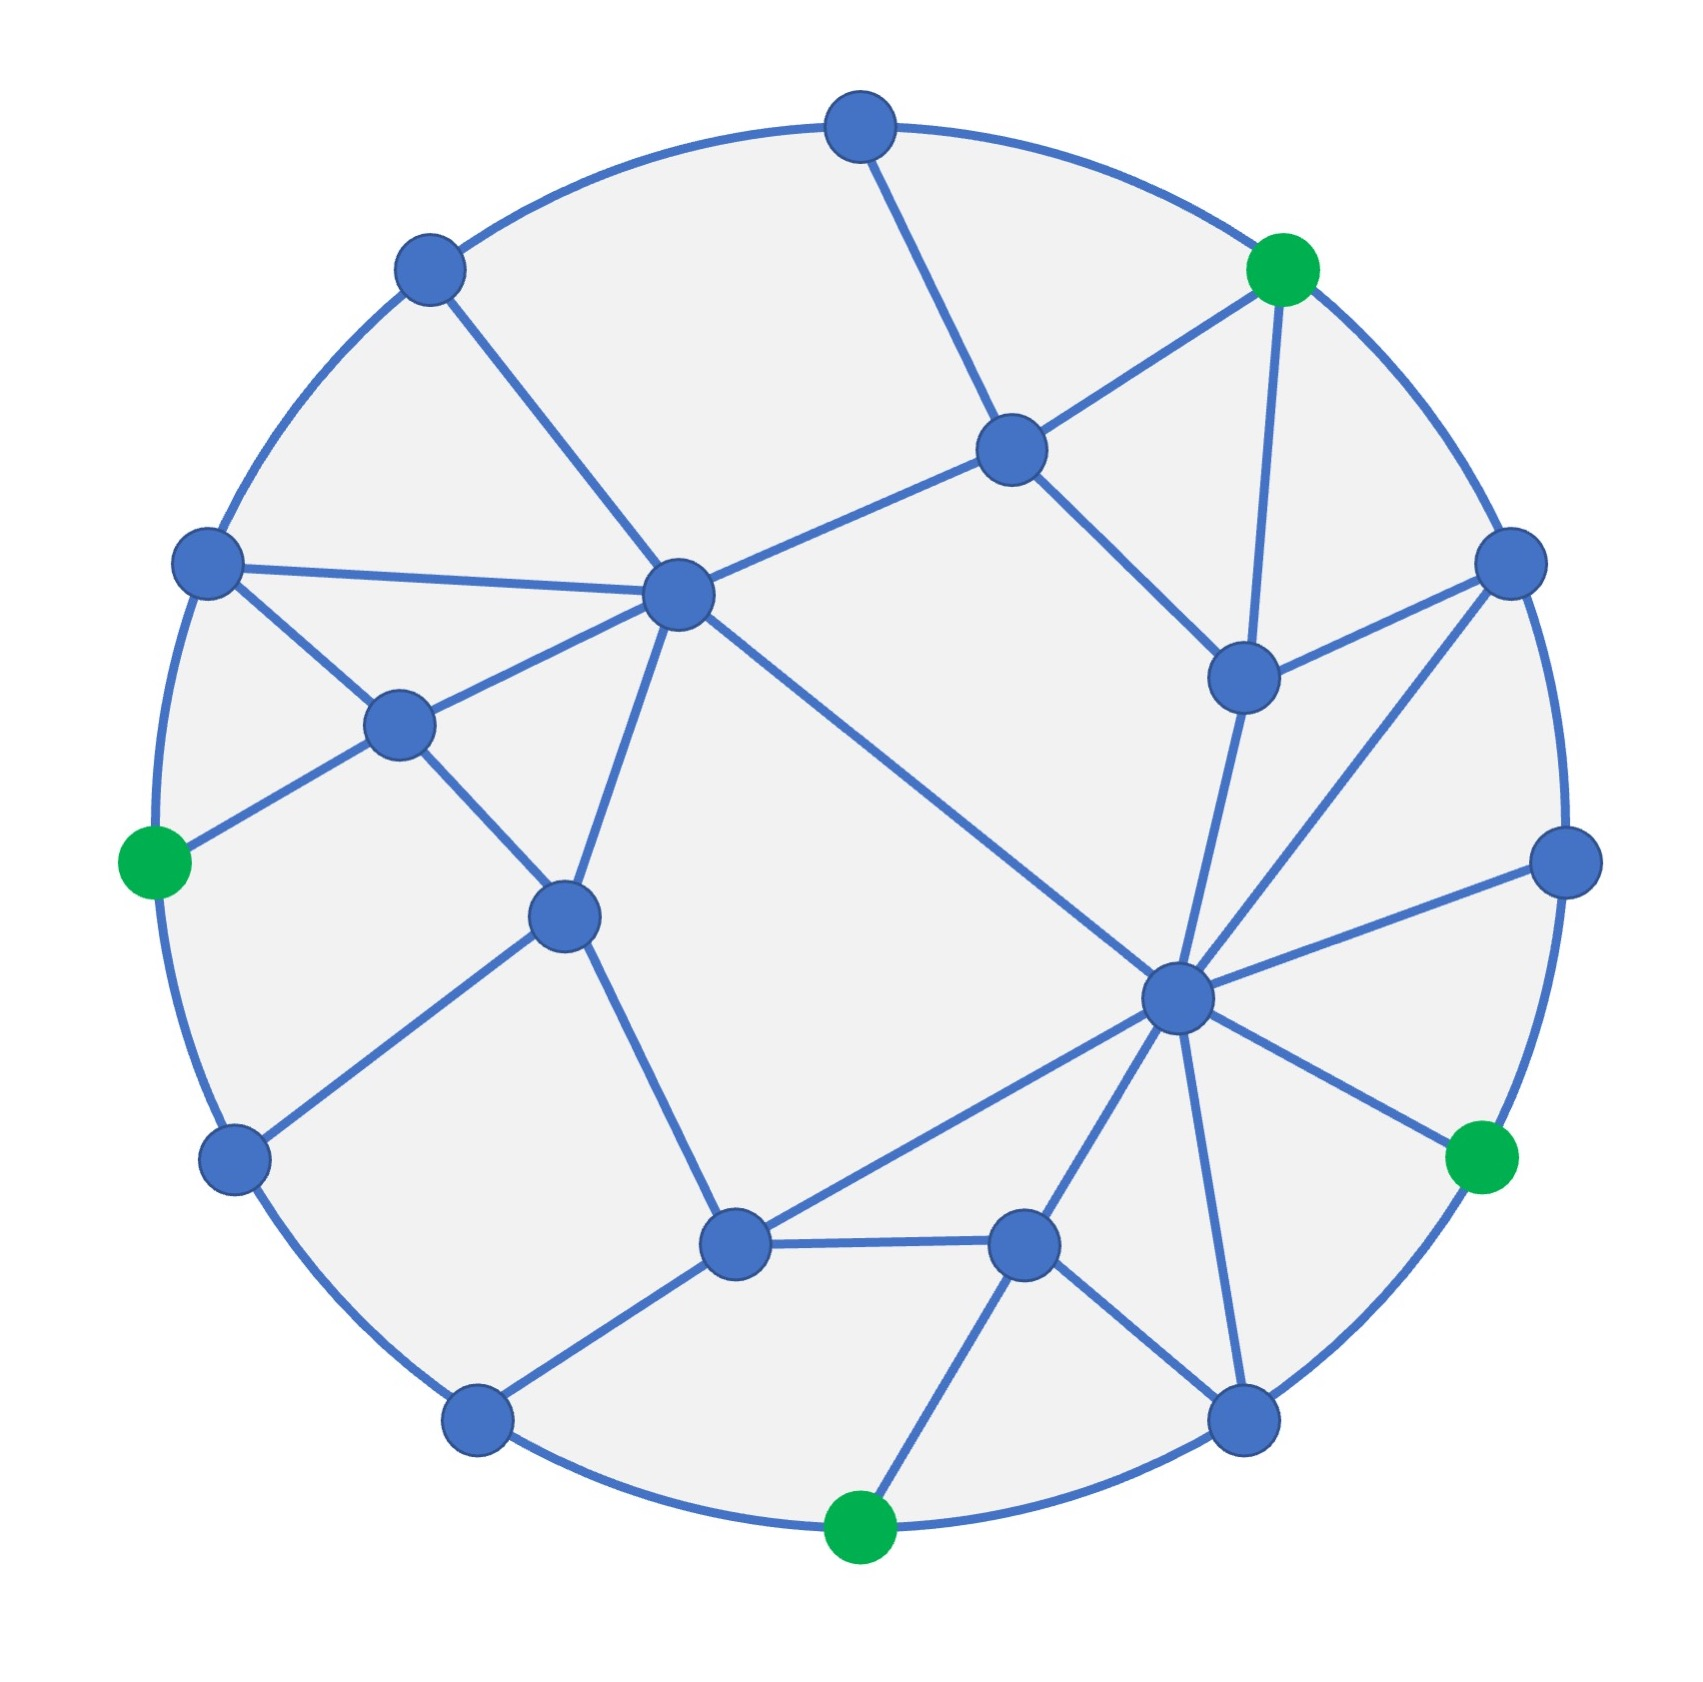
\includegraphics{fig/1face_1}}}
	\hspace{0.7cm}
	\subfigure%[The tight span $\TS(D)$.]
	{
		\scalebox{0.1}{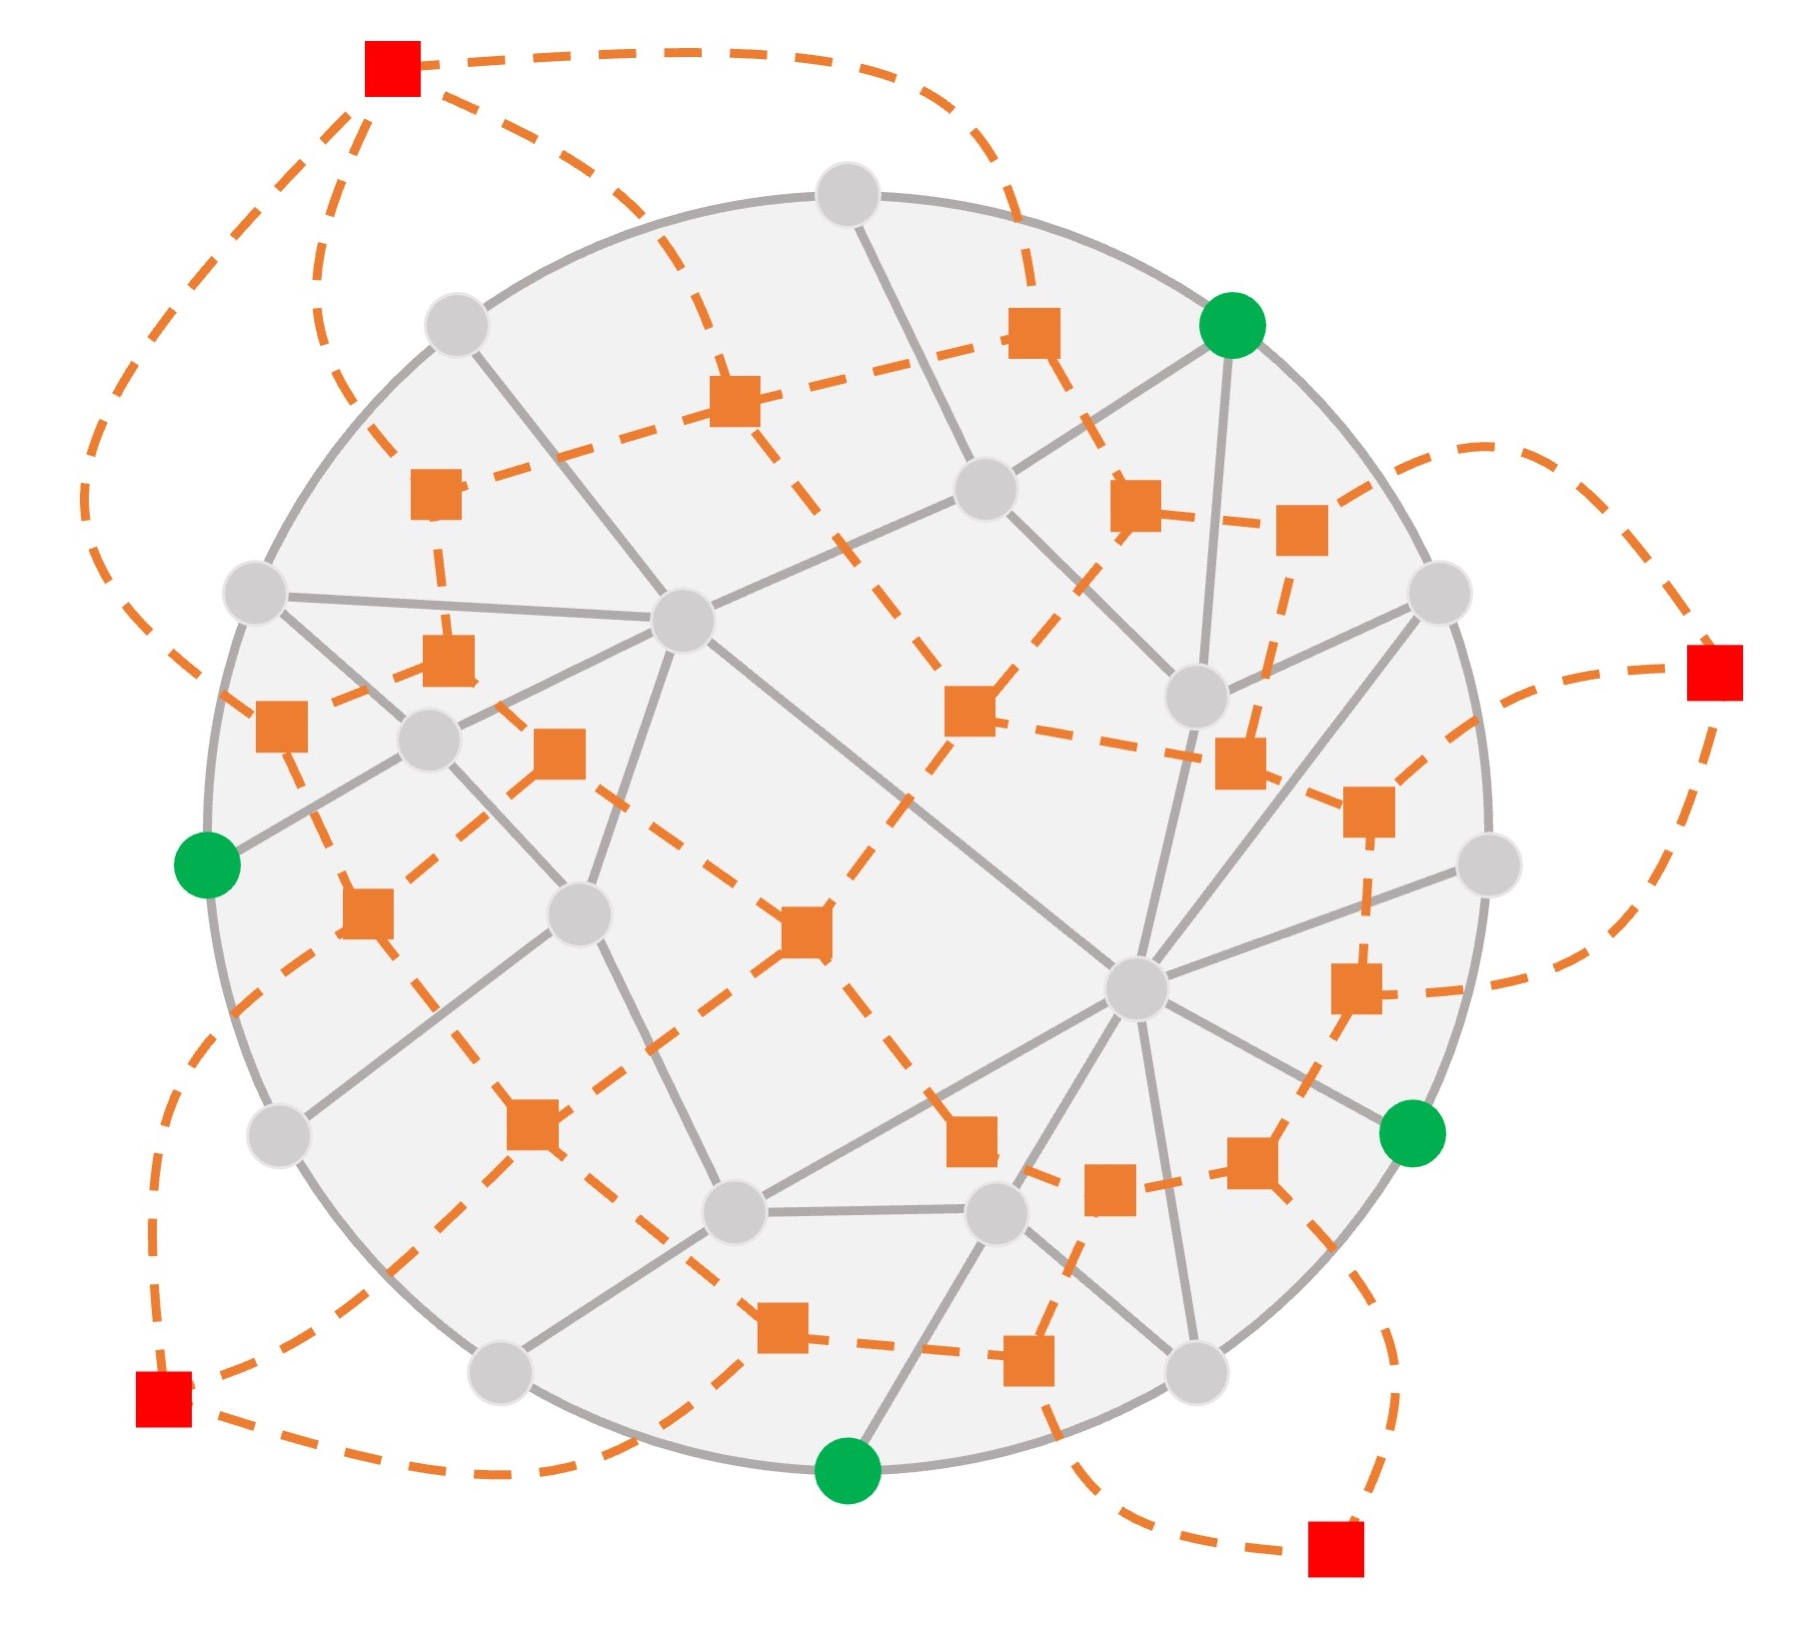
\includegraphics{fig/1face_2}}}
	\caption{An illustration of a one-face instance $(G,T)$ (left) and its dual $(G^*,T^*)$ defined in our way (right). The dual terminals in $T^*$ are marked in red. Taking the dual of (or reverse) $G^*$ we get $G$ back.\label{fig: dual}}
\end{figure}



\subsection{Warm-up: the one-face case}
\label{sec: 1-face}

In this subsection we prove \Cref{main: upper} for the special case where all terminals lie on the boundary of the outer face in the planar embedding of $G$.



\begin{lemma}
	\label{lem: mincut structure}
Let $(G,T)$ be a one-face instance. Then for any partition $(T_1,T_2)$ of the terminals into non-empty subsets, for any min-cut $\hat E$ in $G$ separating $T_1$ from $T_2$, the corresponding edge set $\hat E^*$ in the dual graph $G^*$ is the union of several edge-disjoint shortest paths connecting dual terminals.
\end{lemma}

\begin{proof}\textcolor{red}{TOPROVE 0}\end{proof}


We are now ready to prove \Cref{main: upper} for one-face instances using \Cref{main: upper}.
We first construct the dual graph $G^*$, and use the result in \cite{chang2022near} to construct a quality-$(1+\eps)$ planar distance emulator $\hat G^*$ with size $O(k\cdot \poly(\log k/\eps))$, and then reverse it to get $\hat G$. 
From our definition of dual graphs and their reverse, $\hat G$ contains all terminals and $|V(\hat G)|=O(k\cdot \poly(\log k/\eps))$. It remains to show that $(\hat G,T)$ is a quality-$(1+\eps)$ cut sparsifier for $(G,T)$. 

Let $(T_1,T_2)$ be a partition of $T$.
On the one hand, the min-cut in $G$ separating $T_1$ from $T_2$ consists of several edge-disjoint dual terminal shortest paths in $G^*$, and as $\hat G^*$ is a $(1+\eps)$ aligned distance emulator for $G^*$, we can find, for each such dual terminal shortest path in $G^*$, a shortest path in $\hat G^*$ connecting its corresponding dual terminals, with at most $(1+\eps)$ times the length. By taking the union of the edges in all these paths in $\hat G^*$ (note however that these paths are not necessarily edge-disjoint in $\hat G^*$), we obtain an edge set in $\hat G$ separating $T_1$ from $T_2$ whose value is at most $(1+\eps)$ times the value of $\mc_G(T_1,T_2)$. 
On the other hand, we apply the same analysis, starting with a min-cut in $\hat G$ separating $T_1$ from $T_2$. As $G^*$ is also a $(1+\eps)$ aligned distance emulator for $\hat G^*$, we can derive similarly that $\mc_{\hat G}(T_1,T_2)\le (1+\eps)\cdot \mc_G(T_1,T_2)$.



\subsection{The $O(1)$-face case}

In this subsection we prove the following lemma.

\begin{lemma}
	\label{lem: O(1) face}
	There exists a universal constant $c>0$, such that for any real number $0<\eps<1$, every $f$-face instance $(H,U)$ has an aligned $f$-face instance $(H',U)$ as its quality-$(1+\eps)$ cut sparsifier, with $|V(H')|\le |U|\cdot (cf\log |U|/\eps)^{cf^2}$.
\end{lemma}

Terminal-separating min-cuts in $G$ dual-terminal shortest paths in our graph $G^*$. Therefore, from now on we focus on preserving dual-terminal shortest paths in $G^*$. Recall that $\fset^*$ is the collection of faces in $G^*$ that contains all dual terminals. The following notion is central in our algorithm.


\paragraph{Pattern-shortest paths, pattern distances, and pattern emulators.}
For a pair $t,t'$ of dual terminals in graph $G^*$, there are more than one way for them to be connected by a path, depending on how the path goes around other faces in $\fset^*$, called \emph{patterns},  A rigorous way of defining patterns was given in \cite{krauthgamer2017refined}, which we describe below.

Fix a point $\nu^*$ in the plane.
Let $\gamma$ be a closed curve (not necessarily simple). A vertex $v\notin \gamma$ is said to be \emph{inside} $\gamma$ iff any simple curve connecting $\nu^*$ to $v$ crosses $\gamma$ an odd number of times, otherwise it is said to be \emph{outside} $\gamma$.
%
For a pair $t,t'$ of dual terminals in $G^*$, we denote by $\Pi_{t,t'}$ the shortest path connecting them in $G^*$.
For every face $F\in \fset^*$, we place a point $z_F$ inside its interior. Consider now a path $P$ in $G^*$ connecting $t,t'$. Note that the union of $P$ and $\Pi_{t,t'}$ is a closed curve. Now the \emph{pattern} of $P$ is defined to be a $|\fset^*|$-dimensional vector $\pat(P)=(\phi_F)_{F\in \fset^*}$, where $\phi_F=1$ iff $z_F$ is inside the closed curve formed by the union of $P$ and $\Pi_{t,t'}$ and $\phi_F=-1$ iff $z_F$ is outside.

\begin{observation}
\label{obs: pattern}
Between every pair of terminals there are $2^{f}$ different patterns.
\end{observation}
\begin{proof}\textcolor{red}{TOPROVE 1}\end{proof}

Let $P,P'$ be simple paths with same endpoints, the above definition of pattern implies that paths $P,P'$ \emph{have the same pattern} iff all points $\set{z_F}_{F\in \fset^*}$ lie outside the closed curve $P\cup P'$.
We will also consider paths $P,P'$ with one common endpoint $t$. Let $R$ be a path such that the other-endpoints of $P$ and $P'$ both lie on $R$. In this case we say that paths $P,P'$ have the \emph{same pattern with respect to $R$}, iff all points $\set{z_F}_{F\in \fset^*}$ lie ourside the closed curve formed by the union of $P$, $P'$, and the subpath of $R$ between the other-endpoint of $P$ and the other-endpoint of $P'$.


\iffalse
\begin{observation}
Let $F,F'$ be distinct faces and let $P$ be a path connecting a vertex on face $F$ to a vertex on face $F'$. Let $t,t'$ be terminals such that $\Pi_{t,t'}$ is vertex-disjoint from $P$.
Let $Q$ be any other $t$-$t'$ path with pattern where $\phi_F\ne \phi_{F'}$. Then $Q$ must cross $P$.
\end{observation}
\fi


For a pattern $\pat$, the $t$-$t'$ \emph{$\pat$-shortest path} is defined to be the shortest path among all $t$-$t'$ paths with pattern $\pat$. Its length is defined to be the \emph{$\pat$-distance} between $t,t'$, which we denote by $\dist^{\Phi}(t_1,t_2)$.
Let $(G,T), (H,T)$ be aligned instances. We say that $(H,T)$ is a \emph{quality-$q$ pattern emulator} of $(G,T)$, iff for every pair $t_1,t_2$ of terminals and every pattern $\pat$, the $\pat$-distance between $t_1,t_2$ in $G$ is within factor $q$ from the $\pat$-distance between $t_1,t_2$ in $H$.
We use the following result from \cite{krauthgamer2017refined}.

\begin{theorem}[Adaptation of Theorem 4.6 in \cite{krauthgamer2017refined}]
\label{thm: pattern for cut}
Let $(G,T),(H,T)$ be aligned instances. If the dual instance $(H^*,T^*)$ is a quality-$q$ pattern emulator of the dual instance $(G^*,T^*)$, then $(H,T)$ is a quality-$q$ cut sparsifier of $(G,T)$.
\end{theorem}




\subsection{Constructing pattern emulators}

We will now prove the following lemma, which, combined with \Cref{thm: pattern for cut}, implies \Cref{lem: O(1) face}.

\begin{lemma}
\label{lem: O(1) face emulator}
There exists a universal constant $c>0$, such that for any $0<\eps<1$, every $f$-face instance $(G,T)$ admits a quality-$(1+\eps)$ pattern emulator $(H,T)$ with $|V(H)|\le |T|\cdot (cf\log |T|/\eps)^{cf^2}$.
\end{lemma}

We prove \Cref{lem: O(1) face emulator} by induction on $f$. The base case where $f=1$ has been proved in \Cref{sec: 1-face}.
Assume that we are given a $f$-face instance $(G,T)$.
We will convert it into an $(f-1)$-face instance and apply the inductive hypothesis.
Throughout this subsection, we use the parameters $\eps'=\eps/2f^2$ and $\eps''=(1-1/f^2)\cdot \eps$.

We first pick a pair $t,t'$ of terminals that lie on distinct faces, denoted by $\alpha,\alpha'$, respectively, and compute the shortest path $\Pi_{t,t'}$ in $G$ connecting $t$ to $t'$, such that $\Pi_{t,t'}$ does not contain any terminal as inner vertices. Denote $\Pi=\Pi_{t,t'}$. Then we compute a set of vertices on $\Pi$ that we call \emph{portals}. 

\paragraph{Portals on $\Pi$.}
We use the notion of $\eps$-covers defined in \cite{klein1998fully,thorup2004compact}.
Let $R$ be a shortest path and let $v$ be a vertex that does not lie in $R$. An \emph{$\eps$-cover} of $v$ in $R$ is a set $C(v,R)$ of vertices, such that for any vertex $x\in R$, there exists some $y\in C(v,R)$, such that 
$\dist(v,x)\le \dist(v,y)+\dist(y,x)\le (1+\eps)\cdot\dist(v,x).$
It has been shown \cite{klein1998fully,thorup2004compact} that for every $\eps>0$, shortest path $R$ and vertex $v\notin R$, there exists an $\eps$-cover of $v$ in $R$ of size $O(1/\eps)$.
%
As we want to construct pattern emulators, we will need to modify the definition of $\eps$-covers into a ``pattern version'' accordingly, as follows.

Let $G$ be an $f$-face instance, $R$ be a shortest path in $G$ that does not intersect any face internally, and $v$ be a vertex that does not lie in $R$. 
Let $Q$ be a path connecting $v$ to some vertex in $R$, and let $\Phi$ be its pattern. A \emph{$\Phi$-respecting $\eps$-cover} of $v$ in $R$ is a set $C(v,R,\Phi)$ of vertices, such that for any vertex $x\in R$, there exists some $y\in C(v,R,\Phi)$, such that the shortest $v$-$y$ path with the same pattern as $\Phi$, concatenated with the $y$-$x$ subpath of $R$, is within factor $(1+\eps)$ in length with the shortest $v$-$x$ path with the same pattern as $\Phi$. In other words (slightly abusing the notations),
$$\dist^\Phi(v,x)\le \dist^\Phi(v,y)+\dist(y,x)\le (1+\eps)\cdot\dist^\Phi(v,x).$$
We use the following lemma, whose proof is similar to the previous result of $\eps$-cover and is deferred to \Cref{apd: Proof of lem: pattern cover}.

\begin{lemma}
\label{lem: pattern cover}
For any planar instance $G$, shortest path $R$ in $G$, vertex $v\notin R$, and pattern $\Phi$, there exists a $\Phi$-respecting $\eps$-cover of $v$ in $R$ of size $O(1/\eps)$.
\end{lemma}


We now define a set $Y$ of vertices on $\Pi$ as follows. For each terminal $t$ and for each pattern $\Phi$, let $Y_{t,\Phi}$ be the pattern-respecting $\eps'$-cover of $v$ in $R$ of size $O(1/\eps')$ given by \Cref{lem: pattern cover}. We then let set $Y=\bigcup_{t,\Phi}Y_{t,\Phi}$.
From \Cref{obs: pattern} and \Cref{lem: pattern cover}, 
$|Y|\le O(2^f\cdot |T|/\eps')$.





We then slice the graph $G$ open along the path $\Pi$ connecting faces $\alpha,\alpha'$.
Specifically, we duplicate path $\Pi$ into two copies $\Pi_1,\Pi_2$ and place them closely at two sides (which we call $1$-side and $2$-side, respectively) of its original image, such that the thin strip between them connect faces $\alpha,\alpha'$ into a single face $\beta$.
All vertices $x$ on $P$ into their copies $x_1,x_2$ ($x_1$ lies on $\Pi_1$ and $x_2$ lies on $\Pi_2$), including the terminals $t,t'$ that now have copies $t_1,t_2$ and $t'_1,t'_2$. All weights on edges remain the same. 
It is easy to verify that the obtained graph, which we denote by $G'$, is a $(f-1)$-face instance.
Let $T'$ be the set that contains all copies of terminals and portals in $Y$.
We then construct a quality-$(1+\eps'')$ pattern emulator $H'$ of $G'$ with respect to $T'$, and then glue, for each portal $y\in Y$, its copies $y_1,y_2$ back to their original vertex $y$. The resulting graph is denoted by $H$ and is returned as the pattern emulator for $G$.
For a complete description of the cut and glue operations, please refer to Appendix B of \cite{chang2022near}.
See \Cref{fig: splitting h-hole after} for an illustration.

\begin{figure}[h!]
	\centering
	\subfigure[Graph $G$: faces $\alpha, \alpha'$ (shaded gray), path $\Pi$ (blue), and portals (purple). ]{\scalebox{0.5}{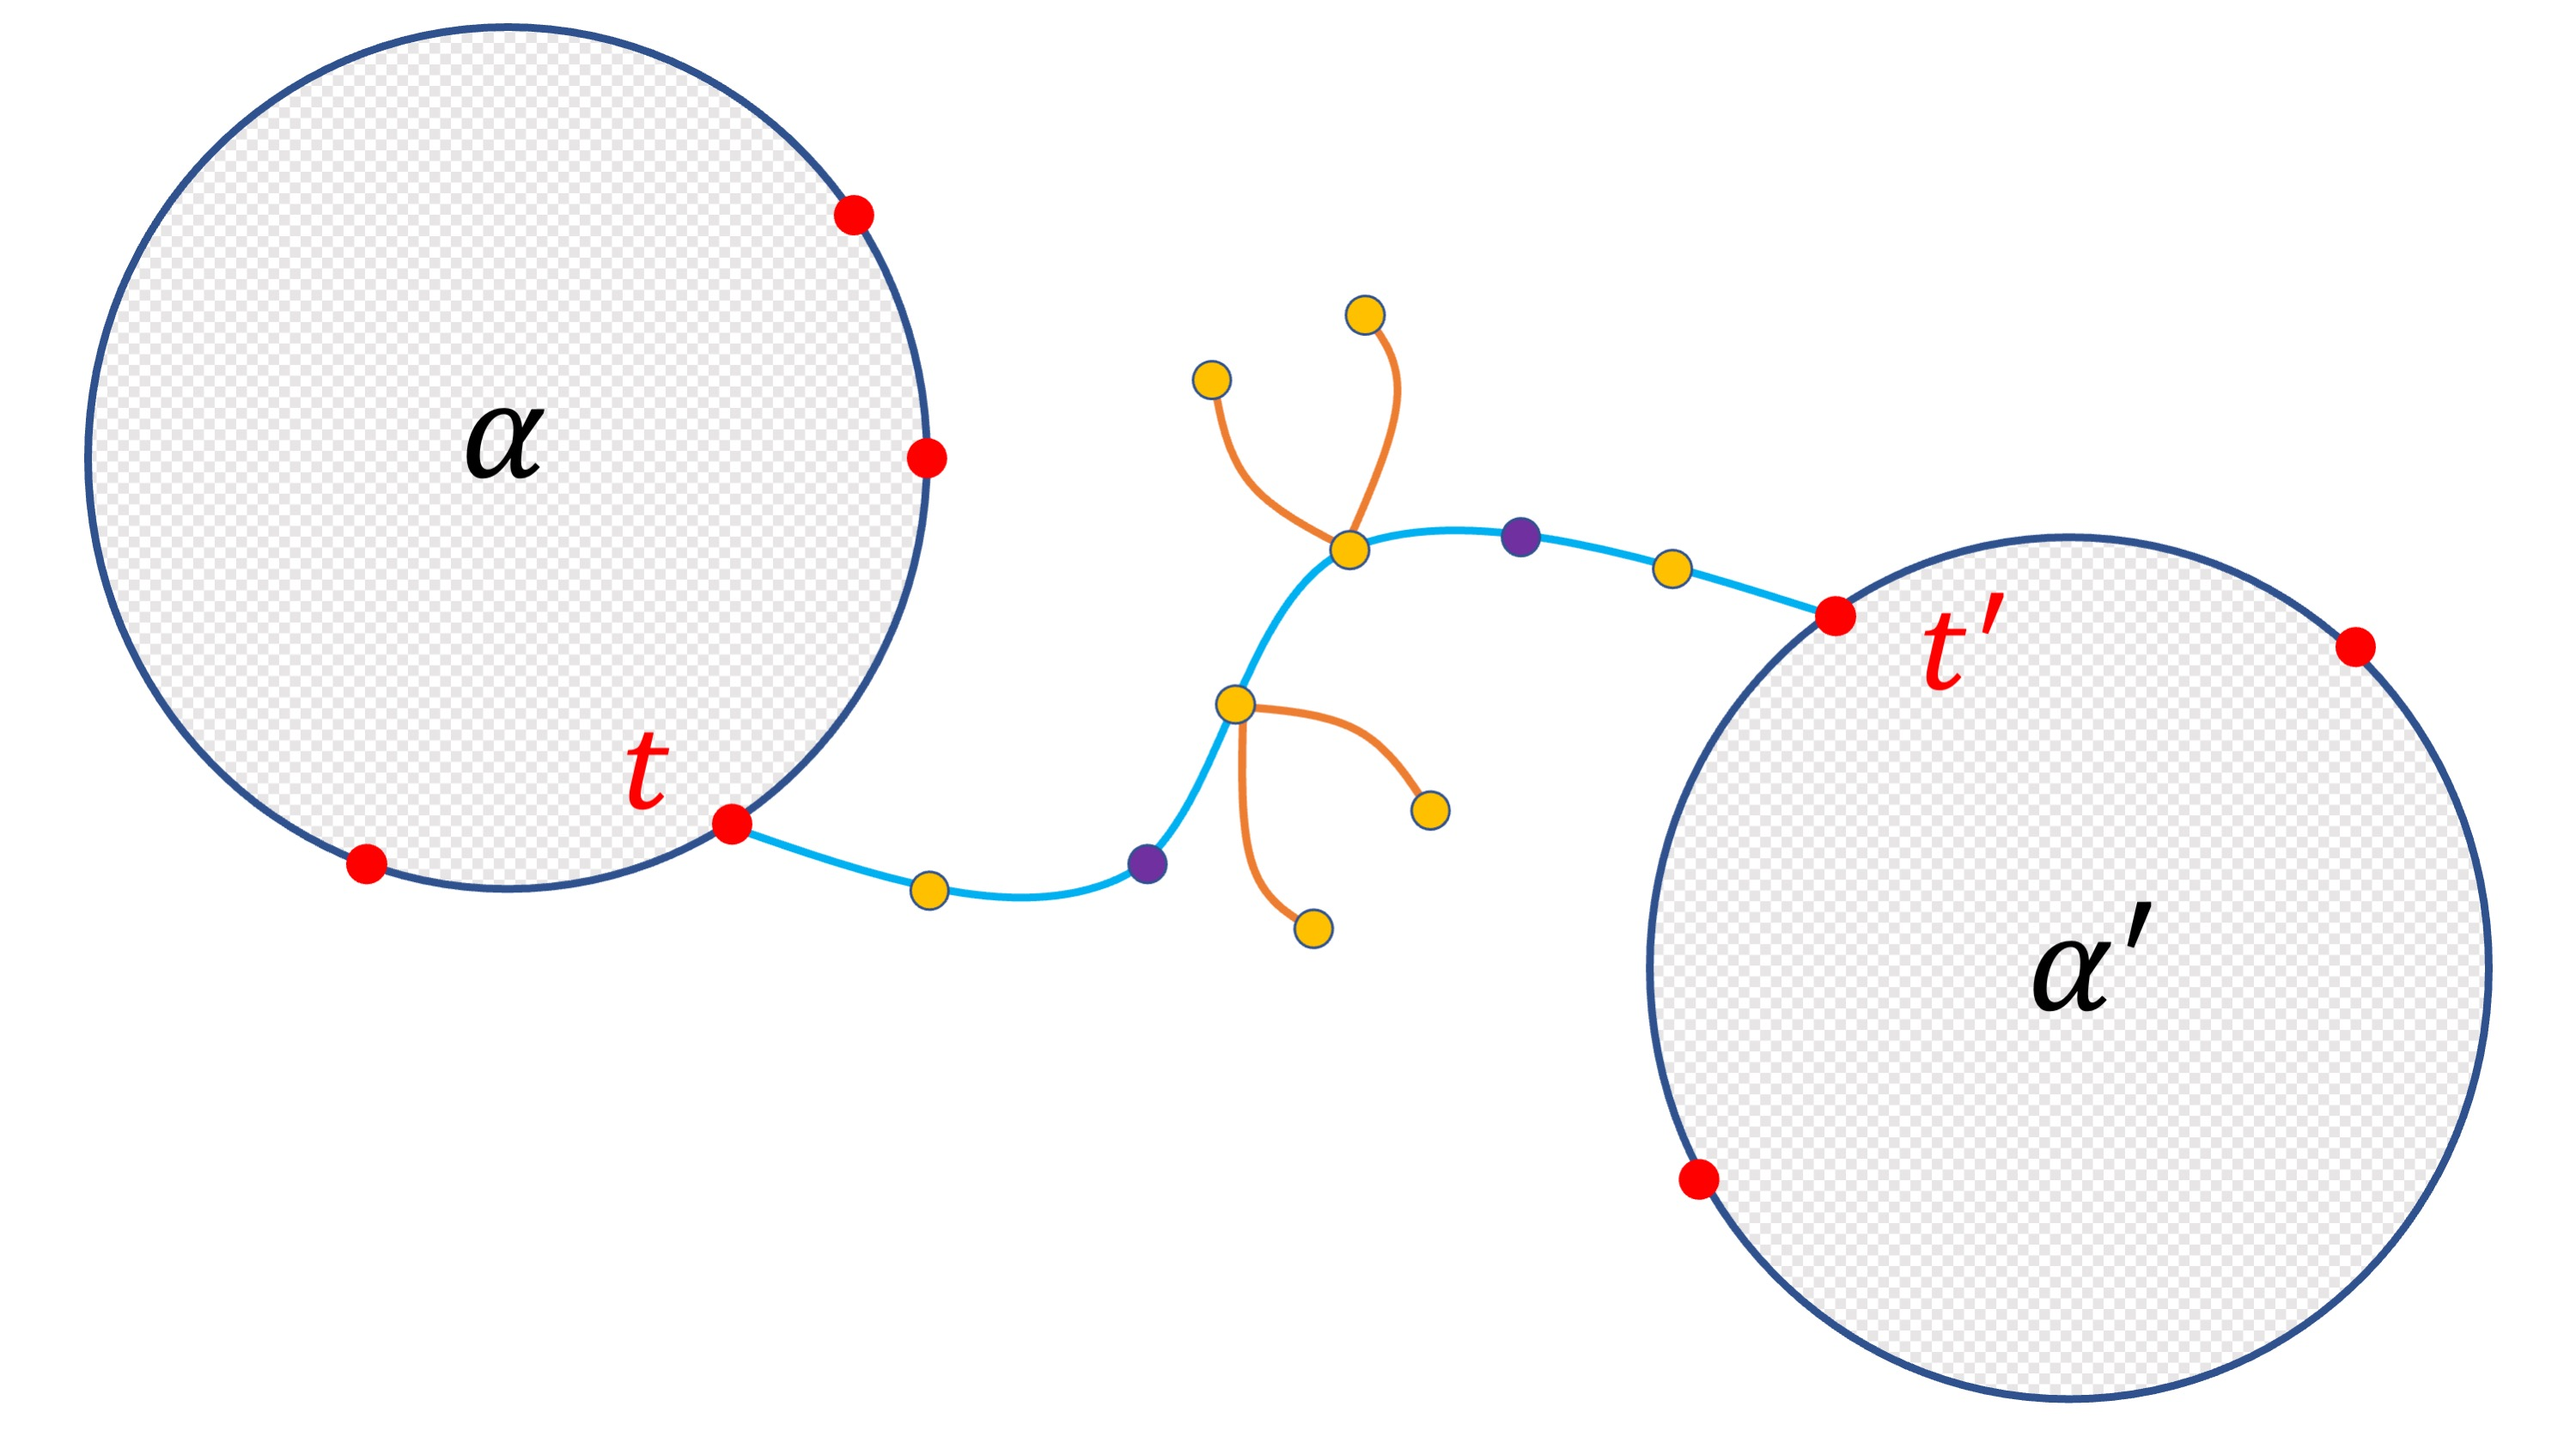
\includegraphics[scale=0.15]{fig/manyhole_1.jpg}\label{fig: splitting h-hole before}}}
	\hspace{0.2cm}
	\subfigure[Graph $G'$: the new hole $\beta$ (shaded gray), and paths $\Pi_1,\Pi_2$ (blue).]{\scalebox{0.5}{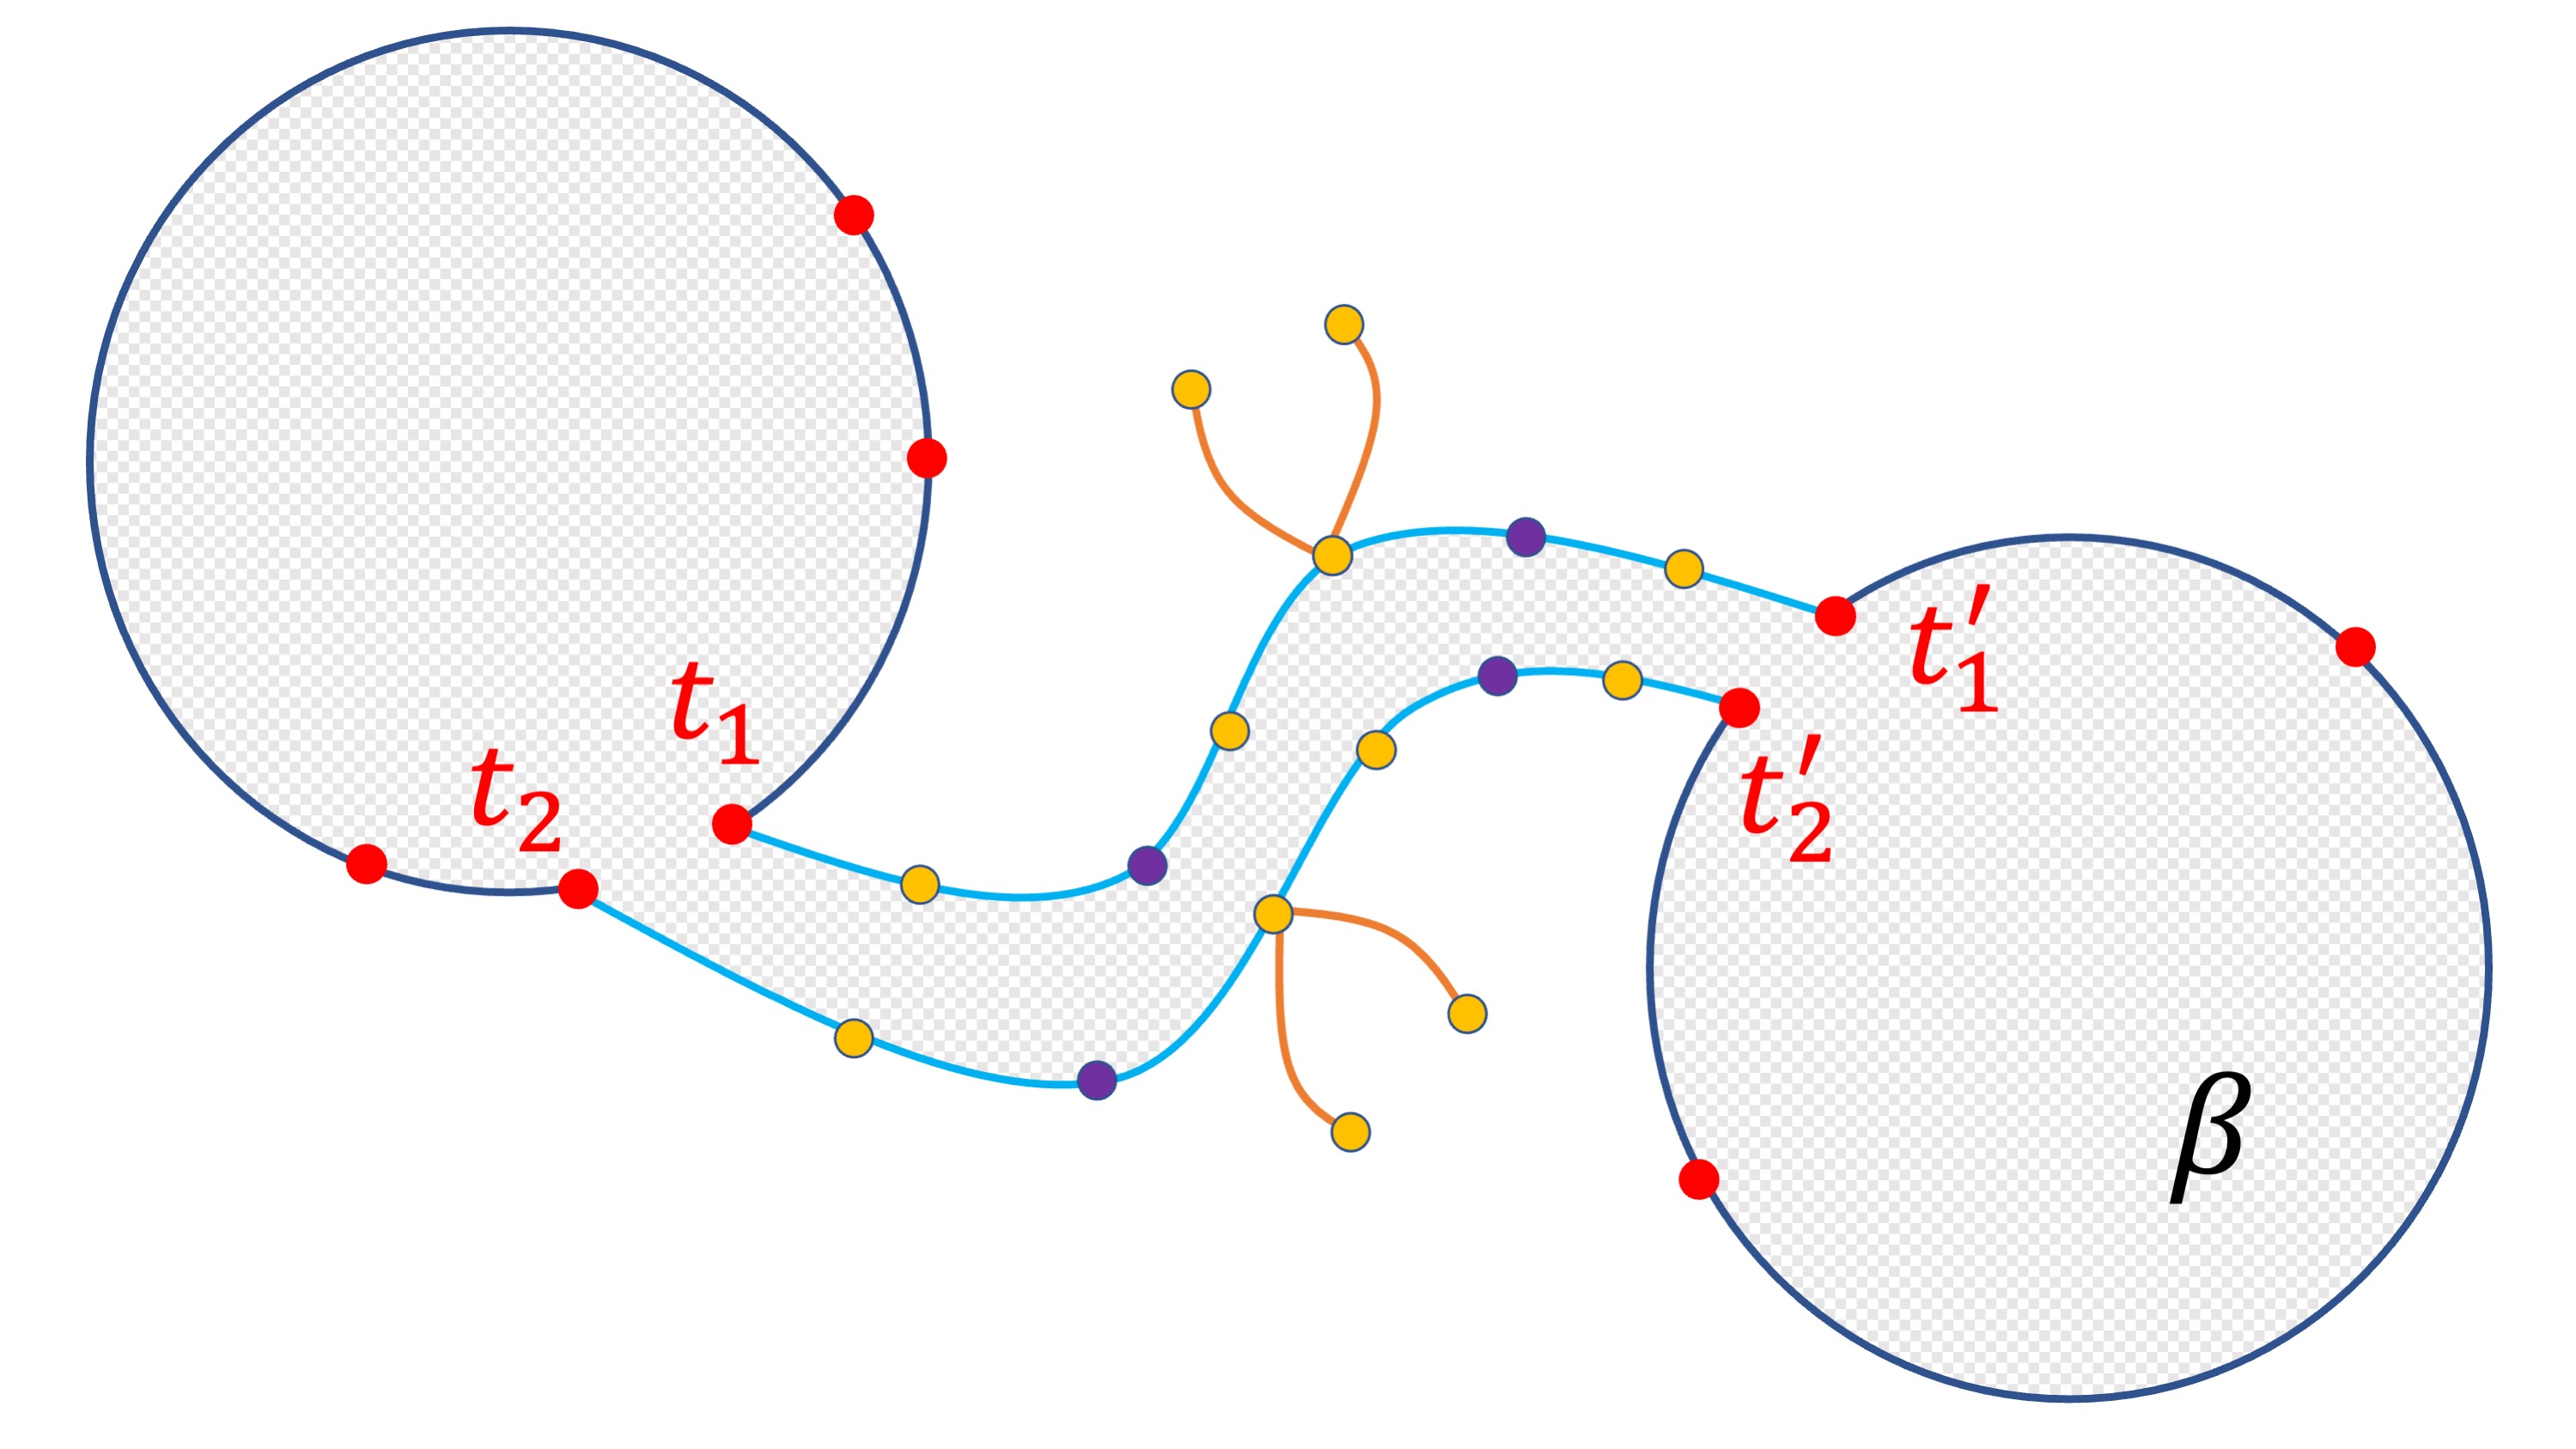
\includegraphics[scale=0.15]{fig/manyhole_2.jpg}\label{fig: splitting h-hole after}}}
	\subfigure[Graph $H$: holes $\alpha,\alpha'$ and portals are restored.]{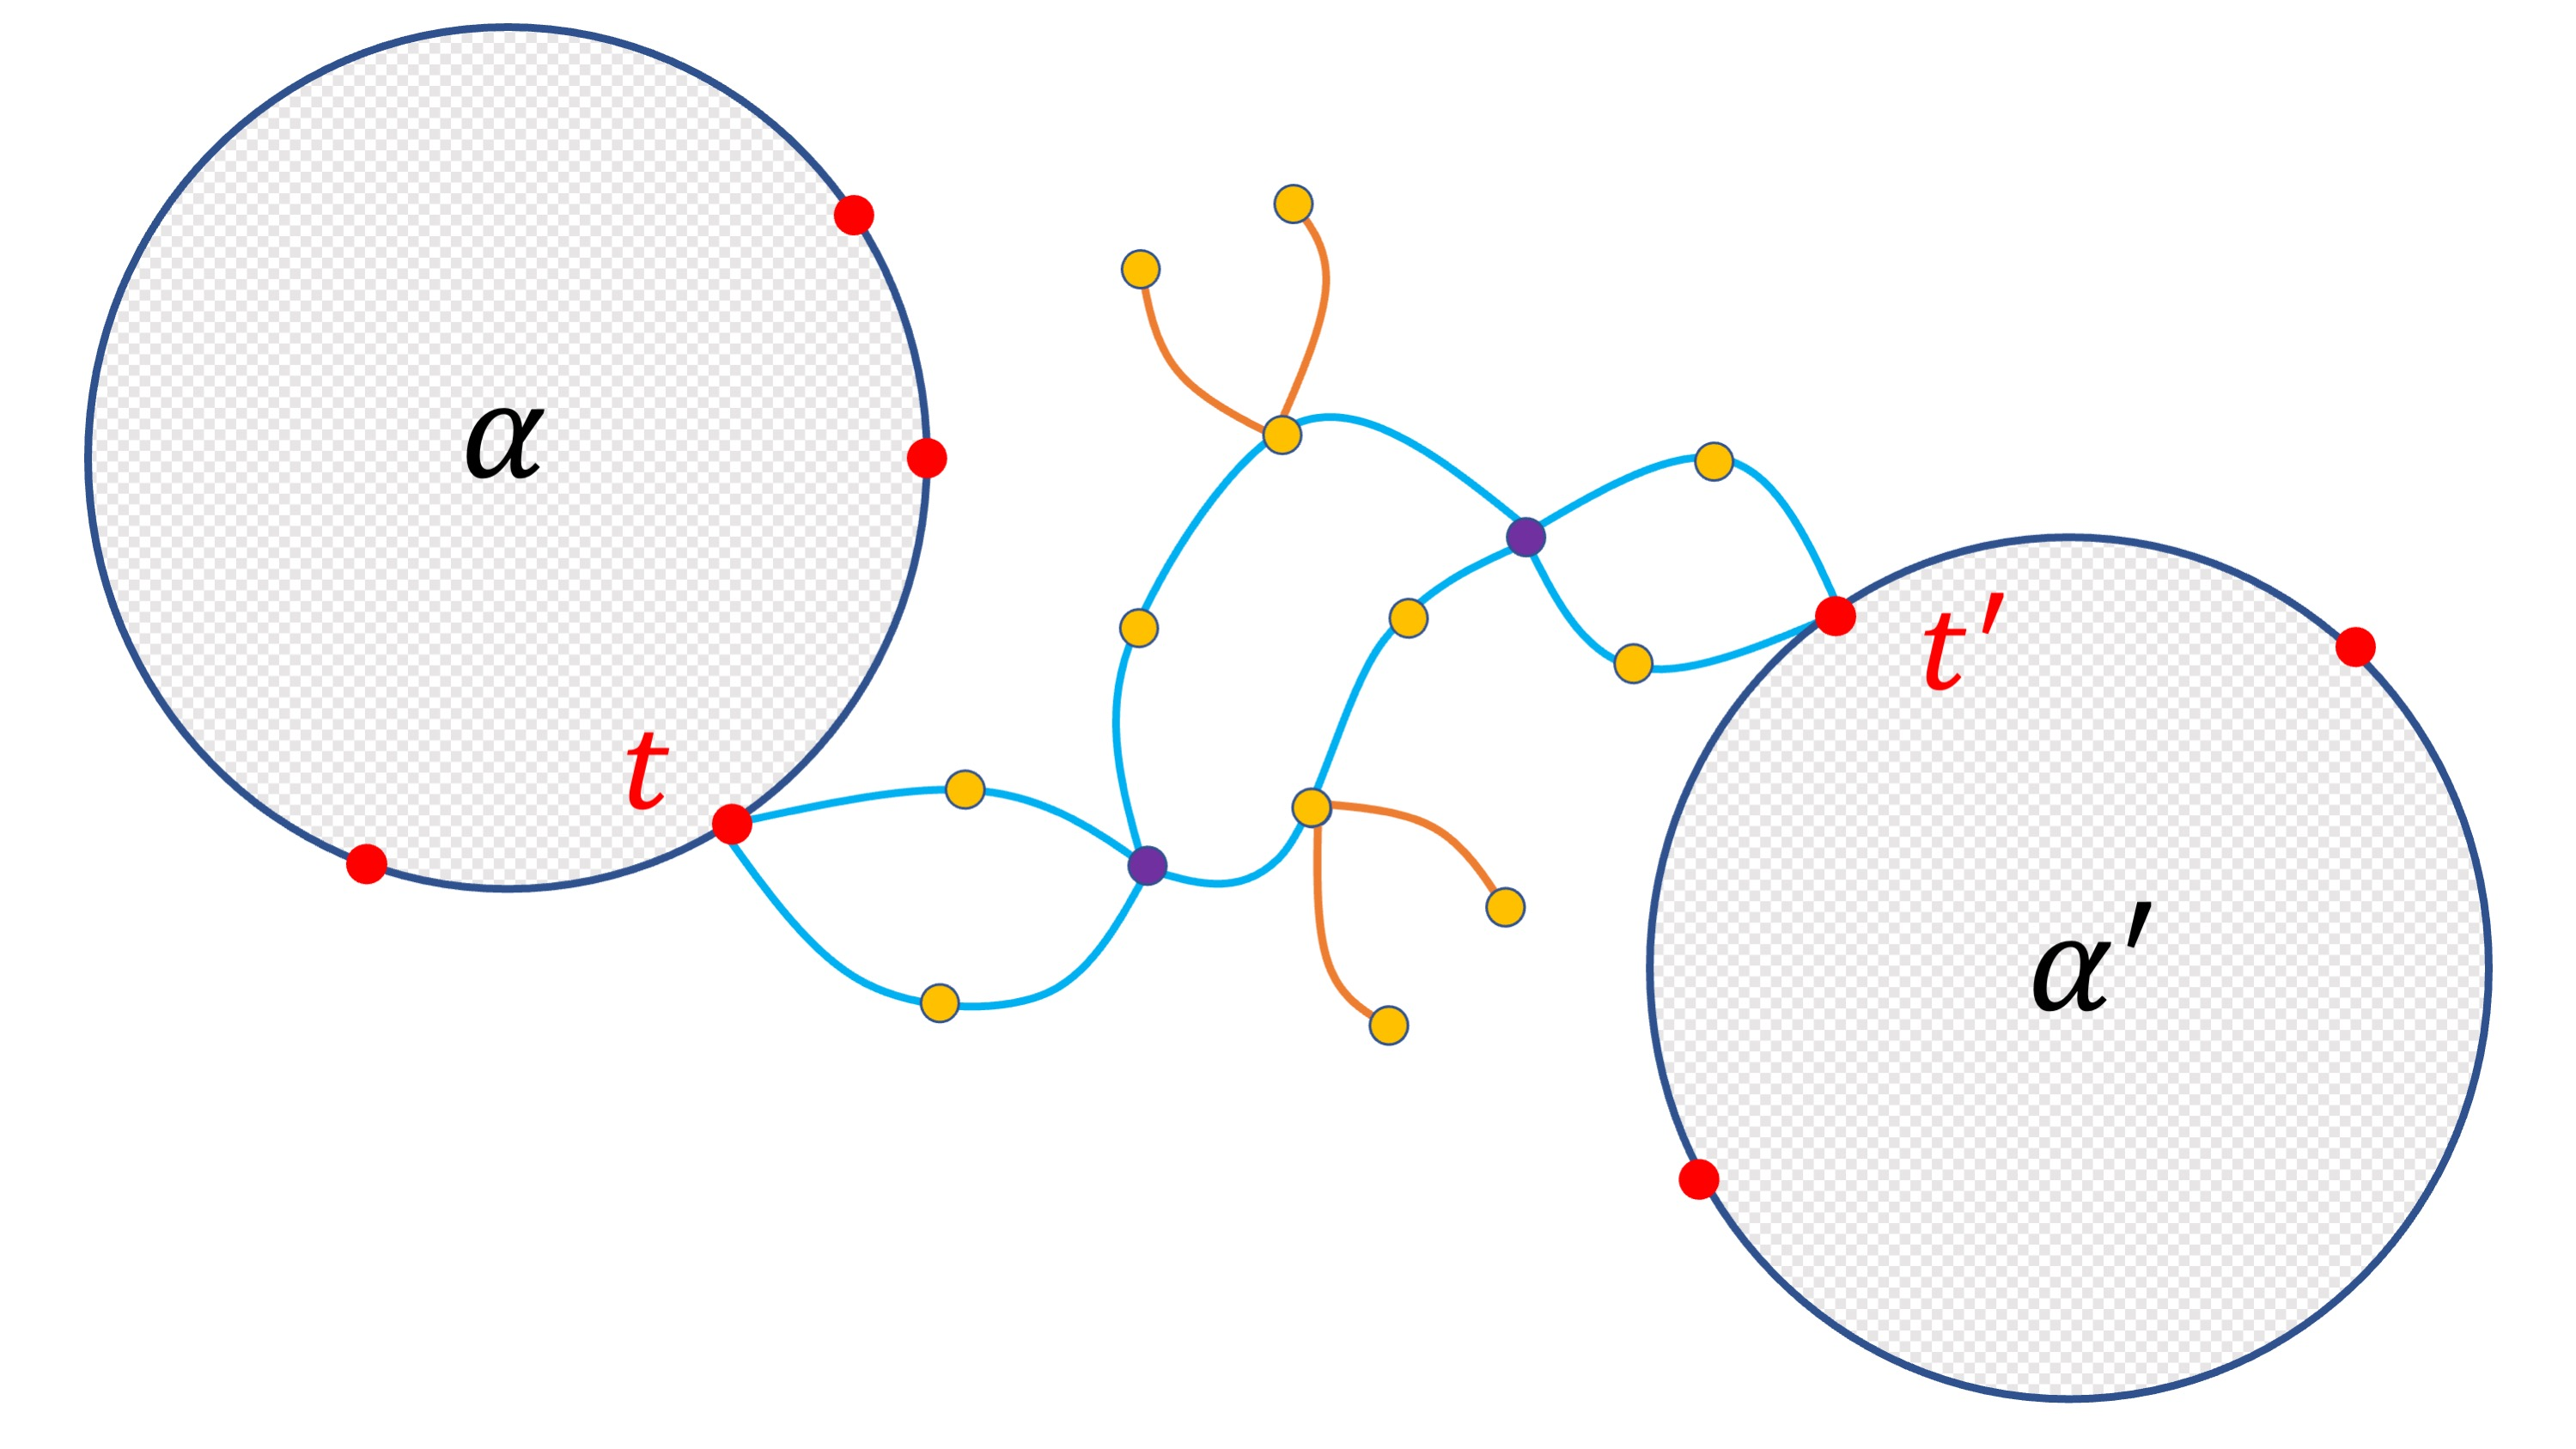
\includegraphics[scale=0.08]{fig/manyhole_3.jpg}\label{fig: gluepath_2}}
	\caption{An illustration of cutting open and gluing an $f$-face instance along path $\Pi$.\label{fig: splitting h-hole}}
\end{figure}




It remains to complete the proof by induction. We first bound the size of graph $H$.
 
\paragraph{Size of $H$.} Since graph $H$ is obtained from graph $H'$ by gluing the portals on paths $\Pi_1,\Pi_2$ back to their original vertices, $|V(H)|\le |V(H')|$, so it suffices to bound the number of vertices in $H'$.
Recall that $T'$ is the set that contains all portals and terminals in $G'$, then
%
\[
\begin{split}
|V(H')| &
\le |T'|\cdot \bigg(\frac{cf\cdot \log |T'|}{\eps''}\bigg)^{c(f-1)^2}
\le \frac{c\cdot 2^f\cdot |T|}{\eps/2f^2}\cdot \bigg(\frac{cf\cdot \log (c\cdot 2^f\cdot |T|/\eps')}{\eps\cdot (1-1/f^2)}\bigg)^{c(f-1)^2}\\
&  \le |T|\cdot \bigg(\frac{cf}{\eps}\bigg)^{c(f-1)^2+f}\cdot \bigg(\frac{\log (cf^2\cdot 2^f\cdot |T|/\eps)}{(1-1/f^2)}\bigg)^{c(f-1)^2}\\
& \le |T|\cdot \bigg(\frac{cf}{\eps}\bigg)^{c(f-1)^2+f}\cdot \bigg(\log |T|+ \log (cf^2\cdot 2^f/\eps)\bigg)^{c(f-1)^2}\\
& \le |T|\cdot \bigg(\frac{cf^2 \log |T|}{\eps}\bigg)^{cf^2},
\end{split}
\]
where we have used the previously set parameters $\eps'=\eps/2f^2$ and $\eps''=(1-1/f^2)\cdot \eps$, and the fact that $(1-\frac{1}{f^2})^{-c(f-1)^2}\le e^{c}< c^{c}$, as $c$ is large enough.



\paragraph{Quality of $H$.}
Recall that we sliced $G$ open along $\Pi$ to obtain $G'$, computed a $(1+\eps'')$ pattern emulator $H'$ for $G'$, and then glue $H'$ back to obtain $H$.
For the purpose of analysis, image that we have also glued $G'$ back to obtain $G''$. The analysis is complete by the following claims.



\begin{claim}
\label{clm: cut glue emulator}
$(H,T)$ is a quality-$(1+\eps'')$ pattern emulator for $(G'',T)$.
\end{claim}
\begin{proof}\textcolor{red}{TOPROVE 2}\end{proof}

\begin{claim}
	\label{clm: cut glue}
	$(G'',T)$ is a quality-$(1+\eps')$ pattern emulator for $(G,T)$.
\end{claim}
\begin{proof}\textcolor{red}{TOPROVE 3}\end{proof}



From \Cref{clm: cut glue} and \Cref{clm: cut glue emulator}, $(H,T)$ is a $(1+\eps'')\cdot (1+\eps')\le (1+\eps)$ pattern emulator for $(G,T)$. This completes the proof by induction of \Cref{lem: O(1) face emulator}.




\subsection{Completing the proof of \Cref{main: upper}}

In this section, we complete the proof of \Cref{main: upper} using the results in previous subsections.

\paragraph{Structured $r$-divisions.} Let $G$ be a planar graph on $n$ vertices and let $T$ be its terminals. For any integer $r>1$, a \emph{structured $r$-division} of $G$ is a collection $\gset$ of subgraphs of $G$, such that
\begin{itemize}
\item $|\gset|=O(n/r)$;
\item the edge sets $\set{E(G')\mid G'\in \gset}$ partitions $E(G)$;
\item for each $G'\in \gset$, $|V(G')|\le r$, $|T\cap V(G')|=O(1+|T|\cdot r/n)$, and if we call vertices in $G'$ that appear in some other graph in $\gset$ its \emph{boundary vertices}, then
\begin{itemize}
\item the number of boundary vertices is $O(\sqrt{r})$;
\item in the planar drawing of $G'$ induced by the planar drawing of $G$, all boundary vertices lie on $O(1)$ faces.
\end{itemize}
\end{itemize}

We use the following lemma in \cite{chang2022near} for computing structured $r$-divisions.

\begin{lemma}[Lemma 5.5 in \cite{chang2022near}]
\label{lem: r-division}
Given any planar instance $(G,T)$ and any integer $r\ge 0$, we can efficiently compute a structured $r$-division.
\end{lemma}

We now prove \Cref{main: upper}. The algorithm is simply: compute a structured $r$-division $\gset$ of the input graph $G$, construct cut sparsifiers for graphs $G'\in \gset$ using \Cref{lem: O(1) face}, and then glue them together to obtain a cut sparsifier for $G$.
It turns out that we need to apply the algorithm several times in order to obtain a near-linear size cut sparsifier, each time with different parameters $r,\eps$.

\begin{lemma}
\label{lem: recursive}
Given any planar instance $(H,U)$ and any $0<\eps<1$, we can efficiently compute a quality-$(1+\eps)$ planar cut sparsifier $(\hat H, U)$ with size $|V(\hat H)|\le O\big(\sqrt{|V(H)| |U|}\cdot (\log |V(H)|/\eps)^{c'}\big)$, for some universal constant $c'>0$.
\end{lemma}

\begin{proof}\textcolor{red}{TOPROVE 4}\end{proof}


We now complete the proof of \Cref{main: upper} using \Cref{lem: recursive}. We start by applying the algorithm in \cite{krauthgamer2017refined} to obtain an exact cut sparsifier $(G_0,T)$ of $(G,T)$ with $|V(G)|=2^{2k}\cdot \poly(k)\le 2^{3k}$.
Then the algorithm consists of two phases.

In the first phase, we set parameters $L=\log k$ and $\eps'=\eps/6L$, and sequentially for each $i=1,\ldots,L$, we apply algorithm \Cref{lem: recursive} to graph $G_{i-1}$ to obtain graph $G_i$.
We show that $|V(G_L)|=(k/\eps)^{O(1)}$ (applying the next lemma with $i=L=\log k$).

\begin{claim}
For each $1\le i\le L$, $|V(G_i)|\le 2^{3k/2^i}\cdot (18k\log k/\eps)^{4c'}$.
\end{claim}
\begin{proof}\textcolor{red}{TOPROVE 5}\end{proof}

In the second phase, we set parameters $\bar L=2\log k\log k$ and $\bar\eps'=\eps/6L$, and sequentially for each $i=1,\ldots,\bar L$, we apply algorithm \Cref{lem: recursive} to graph $G_{L+i-1}$ to obtain graph $G_{L+i}$.

\begin{claim}
	For each $1\le i\le \bar L$, $|V(G_{L+i})|\le k^{1+5c'/2^i}\cdot (5c'\log k/\bar\eps')^{2c'}$.
\end{claim}
\begin{proof}\textcolor{red}{TOPROVE 6}\end{proof}
Applying $i=\bar L$, we get that $|V(G_{L+\bar L})|\le O(k\cdot \poly(\log k/\eps))$ (as $c'$ is a universal constant).

On the other hand, from \Cref{obs: chain}, we get that instance $(G_{L+\bar L},T)$ is a cut sparsifier of  instance $(G,T)$ with quality
$(1+\eps/6L)^L\cdot (1+\eps/6\bar L)^{\bar L}\le (1+\eps)$. The proof is complete.









